\documentclass{article}

% --- FUENTES Y CODIFICACIÓN ---
\usepackage[final,babel=True]{microtype}
\microtypecontext{spacing=nonfrench}
\usepackage{fontspec}
\usepackage{svg}
\usepackage{afterpage}
\svgsetup{inkscapelatex=false,inkscapearea=drawing}
\usepackage{unicode-math}
\setmathfont{Libertinus Math}[Scale=MatchLowercase]
\setsansfont[Scale=MatchLowercase,Ligatures=TeX,
  Extension=.otf,UprightFont=*-Regular,ItalicFont=*-Italic,
  BoldFont=*-SemiBold,BoldItalicFont=*-SemiBoldItalic]{IBMPlexSansCondensed}
\setmonofont[Scale=0.91,Extension=.otf,UprightFont=*-Regular,
  ItalicFont=IBMPlexMono-Italic.otf,BoldFont=IBMPlexMono-Bold.otf,
  BoldItalicFont=IBMPlexMono-BoldItalic.otf]{IBMPlexMono.otf}

% --- IDIOMAS ---
\usepackage[english,portuguese,main=spanish]{babel}
\usepackage[autostyle=true]{csquotes}
\setmainfont[Numbers={OldStyle,Proportional},
  Ligatures={TeX,Common,Discretionary},Scale=1.18]{Libertinus Serif}
\renewcommand{\normalsize}{\fontsize{10pt}{13pt}\selectfont}

% --- BIBLIOGRAFÍA ---
\usepackage[style=apa,backref=true,backend=biber]{biblatex}
\input{/home/solfreitas/.gbpublisher/biblatex/apa-config.tex}


% --- PÁGINA ---
\usepackage[paperwidth=210mm,paperheight=297mm,
  top=13mm,bottom=23mm,left=13mm,right=87mm,
  headsep=0mm,footskip=12mm,headheight=29mm,headsep=10mm,
  marginparsep=6mm,marginparwidth=68mm,
  includehead,includefoot,showframe]{geometry}
\setcounter{secnumdepth}{0}

% --- POSICIONAMIENTO ABSOLUTO ---
\usepackage[absolute,overlay]{textpos}
\setlength{\TPHorizModule}{1mm}
\setlength{\TPVertModule}{1mm}
\textblockorigin{0mm}{0mm}
\newlength{\gbbloquex}
\AtBeginDocument{\setlength{\gbbloquex}{\dimexpr 1in+\hoffset+\oddsidemargin+\textwidth+\marginparsep\relax}}

% --- TABLAS Y FIGURAS ---
\usepackage{booktabs}
\usepackage{graphicx}
\usepackage[labelfont=bf,font=small,labelsep=period,format=plain]{caption}

% --- VARIOS ---
\newcommand{\epigraph}[2]{%
  \par\nobreak\noindent\par\nobreak\vspace{.5\baselineskip}%
  \hfill{%
    \small
    \begin{tabular}{@{}>{{\raggedright\arraybackslash}}m{.65\textwidth}@{}}%
      #1 \\[1ex]%
      \midrule%
      \hfill #2%
    \end{tabular}%
  }%
  \vspace{.5\baselineskip}%
}
\usepackage{hyperref}
\hypersetup{colorlinks=True,linkcolor=azulrevista,citecolor=azulrevista,urlcolor=azulrevista,filecolor=azulrevista,
linktoc=all,breaklinks=True,bookmarksopen=True,bookmarksnumbered=True}
\usepackage[bottom,stable,hang]{footmisc}
\usepackage{scrextend}
\usepackage{changepage}
\newcommand{\fullwidthblock}[1]{%
  \begin{adjustwidth}{0pt}{-\dimexpr\marginparsep+\marginparwidth\relax}%
  \centering #1%
  \end{adjustwidth}%
}
\usepackage{rotating}
\setlength{\footnotesep}{10pt}
\renewcommand{\footnoterule}{%
  \kern -3pt%
  \hrule height 0.5pt width 0.4\columnwidth%
  \kern 6pt}
\renewcommand*{\thefootnote}{\scriptsize\sf{[\arabic{footnote}]}}
\makeatletter
\patchcmd{\@footnotetext}{\footnotesize}{\small}{}{}
\makeatother
\newcommand*\footnotemarkspace{0em}
\deffootnote{\footnotemarkspace}
  {\parindent}
  {\makebox[\footnotemarkspace][r]{\llap{\thefootnotemark\quad}}}
\raggedbottom
\clubpenalty=10000
\widowpenalty=10000
\usepackage{siunitx}
\usepackage{enumitem}
\setlist{nosep,topsep=4pt}
\usepackage{titlesec}
\titleformat{\section}[hang]
  {\sf\bfseries\Large\color{azulrevista}\raggedright}
  {\thesection}{.5em}{}[]
\titlespacing{\section}
  {\parindent}{18pt plus 0.5pt minus 0.5pt}{6.75pt}
\titleformat{\subsection}[hang]
  {\sf\large\color{azulrevista}\raggedright}
  {\thesubsection}{.5em}{}[]
\titlespacing{\subsection}
  {\parindent}{18pt plus 0.5pt minus 0.5pt}{6.75pt}
\titleformat{\subsubsection}[hang]
  {\rm\bfseries\normalsize\color{azulrevista}\raggedright}
  {\thesubsubsection}{.5em}{}[]
\titlespacing{\subsubsection}
  {\parindent}{18pt plus 0.5pt minus 0.5pt}{6.75pt}
\titleformat{\paragraph}[runin]
  {\bfseries\color{azulrevista}}{}{0em}{}[\mbox{ --- }]
\titlespacing{\paragraph}
  {0pt}{6.75pt plus 0.5pt minus 0.5pt}{0pt}
\titleformat{\subparagraph}[hang]
  {\sf\bfseries\large\color{azulrevista}\centering}
  {\thesubparagraph}{.5em}{}[]
\titlespacing{\subparagraph}
  {\parindent}{18pt plus 0.5pt minus 0.5pt}{6.75pt}
% --- COLOR ---
\usepackage[svgnames]{xcolor}
\usepackage{tcolorbox}
\definecolor{azulrevista}{HTML}{2d5a8e}

\usepackage{listings}
\lstset{
  basicstyle=\ttfamily\small,
  breaklines=true,
  breakatwhitespace=false,
  frame=single,
  framerule=0pt,
  backgroundcolor=\color{black!5!white},
  fillcolor=\color{black!5!white},
  rulecolor=\color{black!5!white},
  xleftmargin=8pt,xrightmargin=8pt,
  framexleftmargin=8pt,framexrightmargin=8pt,
  framextopmargin=6pt,framexbottommargin=6pt,
  aboveskip=8pt,belowskip=8pt,
  keywordstyle=\color{blue!70!black}\bfseries,
  commentstyle=\color{green!50!black}\itshape,
  stringstyle=\color{orange!80!black},
  showstringspaces=false,
  numbers=none,
  captionpos=b
}
\renewenvironment{quote}{\normalsize\list{}{\sf\leftmargin=14pt\rightmargin=0pt}\item\relax}{\endlist}

\usepackage[hyphenation,homeoarchy,homeoarchywordcolor=orange,homeoarchycharcolor=orange,draft]{impnattypo}

\renewenvironment{verse}
  {\normalsize\list{}{\leftmargin=14pt\rightmargin=0pt\parsep=0pt}
   \item\relax\itshape}
  {\endlist}
\newcommand{\articulotipo}{}

% --- HEADER / FOOTER ---
\usepackage{fancyhdr}
\setlength{\headwidth}{\textwidth}
\addtolength{\headwidth}{\marginparsep}
\addtolength{\headwidth}{\marginparwidth}

\fancypagestyle{firstpage}{%
  \fancyhf{}%
  \fancyhead[L]{%
    \begin{minipage}[t]{\headwidth}%
    
\includegraphics[width=184mm,height=20mm,keepaspectratio=false]{/home/solfreitas/00_trabajos/00-Demo/media/logo-revista.png}\\[3mm]%
      {\setlength{\fboxsep}{0pt}%
      \colorbox{azulrevista}{%
        \parbox[c][6mm][c]{\headwidth}{%
          \hspace{12pt}\sffamily\bfseries\color{white}\articulotipo%
        }%
      }}%
    \end{minipage}%
  }%
  \renewcommand{\headrulewidth}{0pt}%
  \fancyfoot[L]{%
    \begin{minipage}[t]{\headwidth}%
      \textcolor{azulrevista}{\rule{\headwidth}{1pt}}\\[1pt]%
      \sffamily\thepage\hfill%
      \small\articulorevista{} / e-ISSN: \texttt{\articuloissne}{} / Vol.~\articulovolumen{},~n.\textsuperscript{o}~\articulonumero{} / \articulofecha%
    \end{minipage}%
  }%
  \renewcommand{\footrulewidth}{0pt}%
}%

\pagestyle{fancy}
\fancyhf{}
\fancyhead[L]{%
  \raisebox{\dimexpr\headheight-7mm\relax}[0pt][0pt]{%
    \begin{minipage}[b]{\headwidth}%
      \sffamily\thepage\hfill%
      \small\articulorevista{} / e-ISSN: \texttt{\articuloissne}{} / Vol.~\articulovolumen{},~n.\textsuperscript{o}~\articulonumero{} / \articulofecha\\[1pt]%
      \textcolor{azulrevista}{\rule{\headwidth}{1pt}}%
    \end{minipage}%
  }%
}%
\renewcommand{\headrulewidth}{0pt}

% --- MACROS DEL ARTÍCULO (SOBREESCRITAS POR EL XSLT) ---
\newcommand{\articulotitulo}{}
\newcommand{\articulosubtitulo}{}
\newcommand{\articulotitulotrans}{}
\newcommand{\articuloautores}{}
\newcommand{\articulodoi}{}
\newcommand{\articuloidiomaxml}{es}
\newcommand{\articulorevista}{}
\newcommand{\articuloissne}{}
\newcommand{\articulovolumen}{}
\newcommand{\articulonumero}{}
\newcommand{\articulofecha}{}
\newcommand{\articulopagina}{0}

\begin{document}

\selectlanguage{spanish}

\renewcommand{\articuloidiomaxml}{es}
\renewcommand{\articulotitulo}{Desigualdad digital y rendimiento académico en la educación superior: un estudio comparativo en universidades públicas de Argentina y México}
\renewcommand{\articuloautores}{Sol Freitas}
\renewcommand{\articulodoi}{10.5281}
\renewcommand{\articulotipo}{ARTÍCULO DE INVESTIGACIÓN}
\renewcommand{\articulorevista}{Revista Soma}
\renewcommand{\articuloissne}{2718-8426}
\renewcommand{\articulovolumen}{01}
\renewcommand{\articulonumero}{01}
\renewcommand{\articulofecha}{ 2026}
\renewcommand{\articulopagina}{1}

\setcounter{page}{1}
\thispagestyle{firstpage}

% --- TÍTULO A ANCHO COMPLETO ---
\noindent\begin{minipage}[t]{\dimexpr\textwidth+\marginparsep+\marginparwidth\relax}%
{\sffamily\bfseries\Large\articulotitulo\par}%
\end{minipage}\par
\vspace{3mm}%
\renewcommand{\articulotitulotrans}{Digital Inequality and Academic Performance in Higher Education: A Comparative Study in Public Universities of Argentina and Mexico}
\noindent\begin{minipage}[t]{\dimexpr\textwidth+\marginparsep+\marginparwidth\relax}%
{\sffamily\itshape\normalsize\articulotitulotrans\par}%
\end{minipage}\par
\vspace{4mm}%

% --- BLOQUE LATERAL DE METADATOS ---
\begin{textblock*}{68mm}(\gbbloquex,92mm)
{\setlength{\leftskip}{0pt}\setlength{\parindent}{0pt}%
\noindent\begin{minipage}[t]{68mm}
\sffamily\small\setlength{\parskip}{1pt}
{\bfseries\color{azulrevista}Sol Freitas}\par
{\scriptsize\texttt{\href{https://orcid.org/0009-0007-4821-6354}{https://orcid.org/0009-0007-4821-6354}}}\par
Departamento de Edición\par
\vspace{6pt}
{\bfseries\color{azulrevista!70}Derechos de autor\'ia:}\par
\textcopyright\ 2026 Freitas, S. Publicado por Revista Soma. \par\vspace{6pt}
{\bfseries\color{azulrevista!70}Publicación:} 2026, vol.~01, n\'um.~01, pp.~1--1\par\vspace{6pt}
{\bfseries\color{azulrevista!70}URL:} {\scriptsize\texttt{\href{https://www.google.com/}{https://www.google.com/}}}\par\vspace{6pt}
{\bfseries\color{azulrevista!70}DOI:} {\scriptsize\texttt{\href{https://doi.org/10.5281}{10.5281}}}\par\vspace{6pt}
\vspace{6pt}
{\bfseries\color{azulrevista!70}Compartir:}\par\vspace{3pt}
{\large
\href{https://bsky.app/intent/compose?text=https%3A%2F%2Fwww.google.com%2F}{\includesvg[height=0.9em]{/home/solfreitas/.gbpublisher/fonts/bluesky}}~
\href{mailto:?subject=Desigualdad%20digital%20y%20rendimiento%20acad%C3%A9mico%20en%20la%20educaci%C3%B3n%20superior%3A%20un%20estudio%20comparativo%20en%20universidades%20p%C3%BAblicas%20de%20Argentina%20y%20M%C3%A9xico&body=https%3A%2F%2Fwww.google.com%2F}{\includesvg[height=0.9em]{/home/solfreitas/.gbpublisher/fonts/envelope}}~
\href{https://www.facebook.com/sharer/sharer.php?u=https%3A%2F%2Fwww.google.com%2F}{\includesvg[height=0.9em]{/home/solfreitas/.gbpublisher/fonts/facebook}}~
\href{https://www.linkedin.com/sharing/share-offsite/?url=https%3A%2F%2Fwww.google.com%2F}{\includesvg[height=0.9em]{/home/solfreitas/.gbpublisher/fonts/linkedin}}~
\href{https://www.reddit.com/submit?url=https%3A%2F%2Fwww.google.com%2F&title=Desigualdad%20digital%20y%20rendimiento%20acad%C3%A9mico%20en%20la%20educaci%C3%B3n%20superior%3A%20un%20estudio%20comparativo%20en%20universidades%20p%C3%BAblicas%20de%20Argentina%20y%20M%C3%A9xico}{\includesvg[height=0.9em]{/home/solfreitas/.gbpublisher/fonts/reddit}}~
\href{https://www.researchgate.net/search?q=Desigualdad%20digital%20y%20rendimiento%20acad%C3%A9mico%20en%20la%20educaci%C3%B3n%20superior%3A%20un%20estudio%20comparativo%20en%20universidades%20p%C3%BAblicas%20de%20Argentina%20y%20M%C3%A9xico}{\includesvg[height=0.9em]{/home/solfreitas/.gbpublisher/fonts/researchgate}}~
\href{https://t.me/share/url?url=https%3A%2F%2Fwww.google.com%2F&text=Desigualdad%20digital%20y%20rendimiento%20acad%C3%A9mico%20en%20la%20educaci%C3%B3n%20superior%3A%20un%20estudio%20comparativo%20en%20universidades%20p%C3%BAblicas%20de%20Argentina%20y%20M%C3%A9xico}{\includesvg[height=0.9em]{/home/solfreitas/.gbpublisher/fonts/telegram}}~
\href{https://wa.me/?text=https%3A%2F%2Fwww.google.com%2F}{\includesvg[height=0.9em]{/home/solfreitas/.gbpublisher/fonts/whatsapp}}~
\href{https://twitter.com/intent/tweet?url=https%3A%2F%2Fwww.google.com%2F&text=Desigualdad%20digital%20y%20rendimiento%20acad%C3%A9mico%20en%20la%20educaci%C3%B3n%20superior%3A%20un%20estudio%20comparativo%20en%20universidades%20p%C3%BAblicas%20de%20Argentina%20y%20M%C3%A9xico}{\includesvg[height=0.9em]{/home/solfreitas/.gbpublisher/fonts/x-twitter}}
}\par
\end{minipage}%
}% FIN GRUPO leftskip
\end{textblock*}


\begin{tcolorbox}[colback=brown!8!white,colframe=brown!8!white,boxrule=0pt,arc=2pt,left=4pt,right=4pt,top=3pt,bottom=3pt,before skip=4pt,after skip=4pt]
\begin{otherlanguage}{spanish}
\sffamily\small \textbf{Resumen:} Este estudio analiza la relación entre las condiciones de acceso digital y el rendimiento académico de estudiantes de grado en dos universidades públicas latinoamericanas: la Universidad de Buenos Aires (Argentina) y la Universidad Nacional Autónoma de México. Mediante un diseño de métodos mixtos que combinó una encuesta estructurada (n = 1.247) con entrevistas en profundidad (n = 40), se examinaron cuatro dimensiones de la desigualdad digital: acceso motivacional, acceso material, habilidades digitales y resultados académicos. Los hallazgos muestran que las habilidades digitales constituyen el predictor más fuerte del rendimiento académico y operan como variable mediadora entre el acceso material y los resultados. Las pautas de desigualdad son notablemente similares en ambos contextos nacionales, lo que sugiere determinantes estructurales que trascienden las particularidades locales.
\par\smallskip\noindent\textbf{Palabras clave:} brecha digital, educación superior, desigualdad, habilidades digitales, América Latina
\end{otherlanguage}
\end{tcolorbox}

\begin{tcolorbox}[colback=brown!8!white,colframe=brown!8!white,boxrule=0pt,arc=2pt,left=4pt,right=4pt,top=3pt,bottom=3pt,before skip=4pt,after skip=4pt]
\begin{otherlanguage}{english}
\sffamily\small \textbf{Abstract:} This study examines the relationship between digital access conditions and academic performance among undergraduate students at two Latin American public universities: the University of Buenos Aires (Argentina) and the National Autonomous University of Mexico. Using a mixed-methods design combining a structured survey (n = 1,247) with in-depth interviews (n = 40), four dimensions of digital inequality were examined: motivational access, material access, digital skills, and academic outcomes. Findings show that digital skills are the strongest predictor of academic performance and serve as a mediating variable between material access and outcomes. Inequality patterns are remarkably similar across both national contexts, suggesting structural determinants that transcend local particularities.
\par\smallskip\noindent\textbf{Keywords:} digital divide, higher education, inequality, digital skills, Latin America
\end{otherlanguage}
\end{tcolorbox}

\bigskip
\noindent\rule{\linewidth}{0.4pt}
\bigskip

\section{Introducción}
La expansión del acceso a Internet en América Latina durante las últimas dos décadas ha sido notable en términos cuantitativos, pero insuficiente en su capacidad de reducir las desigualdades estructurales de la región. Los debates iniciales sobre la brecha digital se centraron en la dimensión del acceso físico —la disponibilidad de dispositivos y conectividad—, pero la investigación posterior demostró que las disparidades más significativas se sitúan en las competencias, los usos y los resultados que las personas obtienen de su interacción con las tecnologías \textcite{2563-WARSCHAUER2004,2566-HARGITTAI2002}.

Este desplazamiento conceptual, que van Dijk \textcite{2564-VANDIJK2020} sistematizó en un modelo de cuatro niveles (motivacional, material, de habilidades y de resultados), resulta particularmente relevante para analizar la educación superior. Las universidades públicas latinoamericanas, que atienden a una población estudiantil socialmente heterogénea, se vieron obligadas a adoptar modalidades de enseñanza mediadas por tecnología de manera masiva y abrupta a partir de 2020. Sin embargo, la transición no operó en el vacío: los estudiantes llegaron a ese escenario con dotaciones muy disímiles de recursos digitales.

El presente estudio analiza la relación entre las condiciones de acceso digital de los estudiantes —entendidas en sentido amplio, más allá de la mera conectividad— y su rendimiento académico durante el período 2020-2022 en dos universidades públicas: la Universidad de Buenos Aires (UBA) y la Universidad Nacional Autónoma de México (UNAM). La selección de estos casos responde a su carácter de megauniversidades con poblaciones estudiantiles de extracción social diversa, lo que permite observar la variabilidad interna de la brecha digital en contextos institucionales comparables. :::


\section{De la brecha de acceso a la desigualdad digital}
La noción de “brecha digital” surgió en los años noventa asociada a la preocupación por las disparidades en el acceso a computadoras e Internet entre distintos segmentos de la población. En su formulación más temprana, el problema se concebía en términos binarios: conectados y no conectados. Sin embargo, Hargittai \textcite{2566-HARGITTAI2002} introdujo el concepto de “brecha digital de segundo nivel” para dar cuenta de las diferencias en habilidades y patrones de uso entre quienes ya tenían acceso a la red. Esta distinción abrió un campo de investigación que desplazó el foco desde la infraestructura hacia las prácticas.

Warschauer \textcite{2563-WARSCHAUER2004} profundizó esta línea al proponer un enfoque de inclusión social que integraba recursos físicos, digitales, humanos e institucionales. Desde esta perspectiva, la tecnología no constituye una variable independiente cuyo efecto pueda aislarse, sino que se inscribe en tramas de relaciones sociales que condicionan tanto su apropiación como sus resultados.

Más recientemente, van Dijk \textcite{2564-VANDIJK2020} consolidó un modelo teórico que distingue cuatro tipos de acceso: motivacional (actitudes y disposiciones hacia la tecnología), material (dispositivos, conectividad y sus características), de habilidades (operativas, informacionales, estratégicas) y de resultados (beneficios concretos obtenidos del uso de tecnología). Este modelo permite operacionalizar la desigualdad digital de manera multidimensional y superar las mediciones basadas exclusivamente en la tenencia de dispositivos o la disponibilidad de conexión.


\section{La brecha digital en la educación superior latinoamericana}
En el contexto específico de América Latina, la CEPAL ha documentado extensamente las disparidades en el acceso y uso de tecnologías digitales, señalando que estas reproducen y profundizan desigualdades preexistentes de ingreso, género, etnia y territorio \textcite{2567-CEPAL2021}. La educación superior no escapa a esta dinámica: si bien las tasas de conectividad entre estudiantes universitarios son superiores al promedio nacional en todos los países de la región, las condiciones de ese acceso —calidad de la conexión, tipo de dispositivo, disponibilidad de un espacio adecuado para el estudio— varían enormemente según el origen socioeconómico del estudiante.

Van Deursen y van Dijk \textcite{2565-VANDEURSEN2019} mostraron que la brecha digital de primer nivel se ha desplazado desde las diferencias en el acceso físico hacia las desigualdades en el acceso material: ya no se trata solo de tener o no tener Internet, sino de las condiciones concretas en que se accede. Un estudiante que solo dispone de un teléfono celular con datos móviles limitados enfrenta restricciones cualitativas muy distintas a las de quien cuenta con una computadora de escritorio, conexión de fibra óptica y un espacio privado de trabajo. Estas diferencias, a menudo invisibilizadas por las estadísticas agregadas de penetración de Internet, tienen consecuencias directas sobre las posibilidades de aprendizaje.


\section{Metodología}
Se diseñó un estudio de métodos mixtos con un componente cuantitativo principal y un componente cualitativo complementario. La muestra cuantitativa incluyó 1.247 estudiantes de grado: 623 de la Facultad de Ciencias Sociales de la UBA y 624 de la Facultad de Ciencias Políticas y Sociales de la UNAM, seleccionados mediante muestreo estratificado por carrera y año de cursada durante el segundo semestre de 2022.

Se aplicó un cuestionario estructurado que relevó cuatro dimensiones del acceso digital, operacionalizadas a partir del modelo de van Dijk \textcite{2564-VANDIJK2020}: acceso motivacional (escala de autoeficacia digital, 8 ítems, α = 0,87), acceso material (tipo de dispositivo principal, calidad de conexión, espacio de estudio), habilidades digitales (escala adaptada de van Deursen y van Dijk, \textcite{2565-VANDEURSEN2019}, 12 ítems, α = 0,91) y resultados académicos (promedio ponderado del período 2020-2022, materias aprobadas por semestre). El componente cualitativo consistió en 40 entrevistas semiestructuradas (20 por universidad) con estudiantes que presentaban perfiles contrastantes en las variables de interés.


\section{Condiciones de acceso material}
La Tabla 1 resume las condiciones de acceso material de los estudiantes en ambas universidades. Se observan diferencias significativas tanto entre universidades como entre quintiles de ingreso.


\begin{table}[!ht]
\centering
{\sf\footnotesize\setlength\tabcolsep{4pt}%
  \begin{tabular}{@{}lllll@{}}
    \toprule
    \textbf{\textbf{Indicador}} & \textbf{\textbf{UBA Q1}} & \textbf{\textbf{UBA Q5}} & \textbf{\textbf{UNAM Q1}} & \textbf{\textbf{UNAM Q5}} \\
    \midrule
    Computadora de escritorio o portátil & 42,3 & 96,1 & 38,7 & 94,5 \\
    \midrule
    Conexión fija (fibra o cable) & 51,8 & 93,4 & 35,2 & 91,8 \\
    \midrule
    Espacio privado de estudio & 28,6 & 87,9 & 24,1 & 85,3 \\
    \midrule
    Dispositivo de uso exclusivo & 35,4 & 94,7 & 31,6 & 92,1 \\
    \midrule
    Velocidad ≥ 20 Mbps & 23,1 & 88,2 & 18,4 & 86,7 \\
    \midrule
    Acceso simultáneo sin degradación & 19,7 & 82,5 & 15,3 & 79,8 \\
    \bottomrule
  \end{tabular}
}%
\label{tbl-1}
\end{table}

Los datos revelan una pauta consistente: mientras que los estudiantes del quintil más alto presentan condiciones de acceso material prácticamente universales en ambas universidades, los del quintil más bajo enfrentan restricciones severas en todos los indicadores. La brecha es particularmente pronunciada en la disponibilidad de espacio privado de estudio y en la velocidad de conexión, dos factores que la literatura identifica como determinantes para el aprovechamiento académico de las herramientas digitales.


\section{Habilidades digitales y rendimiento académico}
El análisis de regresión múltiple mostró que las habilidades digitales, medidas mediante la escala adaptada, constituyen el predictor más fuerte del rendimiento académico en el período analizado (β = 0,34; p < 0,001), por encima del acceso material (β = 0,21; p < 0,01) y del acceso motivacional (β = 0,18; p < 0,01). Sin embargo, el análisis de mediación reveló que las habilidades digitales operan, en buena medida, como variable mediadora entre el acceso material y el rendimiento: los estudiantes con mejores condiciones materiales desarrollan habilidades digitales más sofisticadas, lo que a su vez se traduce en mejores resultados académicos.

La Figura 1 presenta el modelo de mediación estimado con las cargas estandarizadas.


\begin{tcolorbox}[colback=white,colframe=azulrevista,leftrule=3pt,rightrule=0pt,toprule=0pt,bottomrule=0pt,arc=0pt,left=8pt,right=4pt,top=3pt,bottom=3pt,before skip=4pt,after skip=4pt]
{\sffamily\small

\begin{figure}[!ht]
\centering
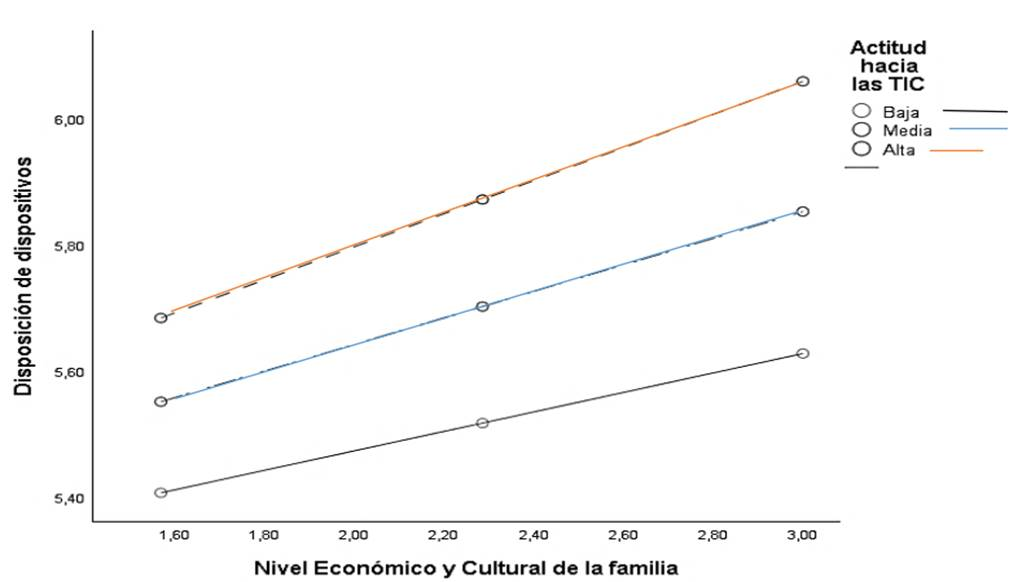
\includegraphics[width=\linewidth]{../media/Figura1.png}
\captionof{figure}{Modelo de mediación con cargas estandarizadas}
\vspace{\intextsep}
\end{figure}

\textbf{Figura 1.} Modelo de mediación entre acceso material, habilidades digitales y rendimiento académico. Coeficientes estandarizados; *p < 0,05; **p < 0,01; ***p < 0,001.

}
\end{tcolorbox}

Experiencias de la brecha: evidencia cualitativa

Las entrevistas en profundidad permitieron iluminar los mecanismos concretos a través de los cuales opera la desigualdad digital en la vida cotidiana de los estudiantes. Un hallazgo recurrente fue lo que denominamos “gestión del ancho de banda doméstico”: en hogares donde varios miembros comparten una única conexión, los estudiantes desarrollan estrategias de negociación del uso de Internet que incluyen cursar en horarios de baja demanda, desactivar la cámara durante las clases sincrónicas para reducir el consumo de datos o descargar materiales en horarios nocturnos.

Otro hallazgo relevante fue la relación entre el tipo de dispositivo y las prácticas de escritura académica. Los estudiantes que accedían predominantemente desde teléfonos móviles reportaron dificultades significativas para la redacción de trabajos extensos, la consulta simultánea de múltiples fuentes y el uso de herramientas de gestión bibliográfica. Estas restricciones operativas se traducían, según los entrevistados, en entregas de menor calidad y en una percepción de desventaja respecto de sus compañeros con mejores condiciones de equipamiento.


\section{Discusión}
Los resultados de este estudio confirman la pertinencia del modelo multidimensional de van Dijk \textcite{2564-VANDIJK2020} para analizar la desigualdad digital en contextos educativos latinoamericanos. La brecha entre los quintiles extremos de ingreso no se limita a la conectividad —que, aun siendo desigual, ha mejorado significativamente— sino que se extiende a las condiciones materiales del acceso, las habilidades digitales y, en última instancia, los resultados académicos.

El efecto mediador de las habilidades digitales sobre la relación entre acceso material y rendimiento coincide con lo reportado por Hargittai \textcite{2566-HARGITTAI2002} en contextos del norte global y sugiere que las políticas de inclusión digital que se limitan a la provisión de dispositivos y conectividad resultan necesarias pero insuficientes. Sin intervenciones específicas orientadas al desarrollo de competencias digitales —no solo instrumentales sino también informacionales y estratégicas—, el acceso material no se traduce automáticamente en mejores oportunidades educativas.

La comparación entre la UBA y la UNAM muestra pautas notablemente similares en ambos contextos, lo que sugiere que la desigualdad digital en la educación superior responde a factores estructurales que trascienden las particularidades nacionales. En ambos casos, la variable con mayor poder discriminante es el origen socioeconómico del estudiante, que condiciona simultáneamente las distintas dimensiones del acceso digital. Este hallazgo es consistente con la tesis de la CEPAL sobre la reproducción digital de la “matriz de la desigualdad social” latinoamericana \textcite{2567-CEPAL2021}.


\section{Conclusiones}
Este estudio aporta evidencia empírica sobre la naturaleza multidimensional de la desigualdad digital en la educación superior latinoamericana. Los datos muestran que, incluso en universidades públicas con políticas activas de inclusión, las condiciones de acceso digital de los estudiantes reproducen las desigualdades socioeconómicas de origen y se traducen en disparidades académicas mensurables.

Las implicancias para la política universitaria son claras: las estrategias de virtualización o hibridación de la enseñanza deben acompañarse de programas integrales que aborden simultáneamente la provisión de equipamiento, la conectividad, el desarrollo de habilidades digitales y la adaptación de las prácticas pedagógicas a contextos de acceso heterogéneo. De lo contrario, la digitalización de la educación superior corre el riesgo de convertirse en un mecanismo adicional de reproducción de la desigualdad.



\end{document}
